\documentclass[a4paper,12pt]{article}

\usepackage{amsmath,amssymb,amsfonts,amsthm}    	% Typical maths resource packages
\usepackage{graphicx}                          							 % Packages to allow inclusion of graphics
\usepackage{hyperref}                           							% For creating hyperlinks in cross references
\usepackage{booktabs}
\usepackage[authoryear]{natbib}                						 % literature reference style
\usepackage[bf]{caption2}
\usepackage{lscape}
\usepackage[hang,flushmargin]{footmisc} 
\usepackage{float}
%\usepackage[german]{babel}
% -------------------------------
% --- some layout definitions ---
% -------------------------------

% define topline
\usepackage[automark]{scrpage2}
\pagestyle{scrheadings}
\automark{section}
\clearscrheadings
\ohead{\headmark}
\cfoot{\thepage}


\usepackage{listings}
%-----------------FRANZISKA
\usepackage{subfigure} 		%für Bilder nebeneinander
\usepackage{wrapfig}		%textumflossene Bilder
\usepackage{graphicx} 		%um \includegraphics[width=0.9\textwidth]{Bild_Name.jpg} verwenden zu können
\setlength{\parindent}{0pt} % damit nach Absatz nicht eingrückt wird
\usepackage{setspace}
\captionsetup{margin=15pt, font={small,stretch=1}, singlelinecheck=false}
%----------------------------FRANZISKA 2

\usepackage[T1]{fontenc}
\usepackage[english]{babel}
\usepackage{listings}
\usepackage{xcolor}
\usepackage{eso-pic}
\usepackage{mathrsfs}
\usepackage{url}
\usepackage{amssymb}
\usepackage{amsmath}
\usepackage{multirow}
\usepackage{hyperref}
\usepackage{booktabs}

\usepackage{cooltooltips}
\usepackage{colordef}
\usepackage{lvblisting}
%------------------------------------------			
							
% define citation style
\bibliographystyle{ecta} %bibliography style of Econometrica

% define page size, margin size
\setlength{\headheight}{1.1\baselineskip}
\voffset=-3cm
\hoffset=-3cm
\textheight24cm
\textwidth16.5cm
\topmargin2.5cm
\oddsidemargin3.5cm
\evensidemargin2.5cm

% define line line spacing = 1.5 or =2
\renewcommand{\baselinestretch}{1.5} %doublespacing

% define second level for `itemizing'
\renewcommand{\labelitemii}{-}

%--------------------DAMIANO Theorems
\newtheorem{definition}{Definition}[section]
\newtheorem{theorem}{Theorem}[section]
%------------------------------------

\begin{document}

\thispagestyle{empty}
\begin{center}

    {\Large{\bf Predicting return probabilities of an online retailer by machine learning algorithms}} \vspace{0.5cm}


    {\normalsize by \\\vspace{0.5cm}
    {\bf Ferrari, Damiano \#591538 \\
    Haeusler, Konstantin \# 551078 \\
    Wehrmann, Franziska \#592500} \\
    } \vspace{1cm}

	{	
\includegraphics[scale=0.2]{logo_hu.png}}

	\vspace{1cm}	
	
    {\normalsize Statistical Programming Languages \\
    Ladislaus von Bortkiewicz Chair of Statistics \\
    Tutor: Alla Petukhina \\
    Humboldt University Berlin \\
    Berlin,  March 14, 2018}

\end{center}


\newpage

\section{Introduction}

Recently, the market share of online retailers increased drastically. The economic importance of this sector is reflected in the growth of revenues generated by online retailers: from 24.6 billion Euro in 2012 to 52.8 billion Euro in 2015 (which represents 1.5\% of the German GDP at that time)\footnote{Revenues of Online Retailers in Germany 2015, source: https://de.statista.com/statistik \\ /daten/studie/29201/umfrage/umsatz-im-online-handel-in-deutschland-seit-2008/}. This development is accompanied by huge logistic efforts. To avoid undesired shipping costs, one challenge of corporate data mining is to reduce these costs to a minimum.

Several papers have outlined the importance of data mining in supporting managerial decision making \cite{manyika2011}. There is a broad literature about each step of the data mining process, from data preprocessing \cite{crone2006} to the design of data mining algorithms \cite{lessmann2015}. The research in this area is undergoing massive transformations due to technological and methodological innovations, e.g. modern storage capacities allow to process huge amounts of data and new statistical methods evolve in order to analyze this data adequately. \\
In this seminar paper, a case study is presented that comprises the essential tools of corporate data mining in the context of online marketing. A raw data set of an online retailer with 150.000 observations and 13 variables is given; for two thirds of the observations exists a binary 'return'-variable $y \in \{0,1\}$ that indicates if a product has been returned by the customer to the retailer (hereafter referred as \textit{known}). The task is to train a model that predicts with high accuracy whether a product of the last third (hereafter referred as \textit{unknown}) of the data set is likely to be returned or not. In order to support the managerial decision making, these predictions are then used to minimize a loss function that consists of type one error $\mathbb{P}(\hat{y}=1|y=0)$ and a type two error $\mathbb{P}(\hat{y}=0|y=1)$.  \\

\begin{table}[h]
 \begin{tabular}{l  l | l l}
  & & & \textbf{True Value} \\
  & & item kept (0) & item returned (1) \\
  \hline
  \textbf{Prediction} & item kept (0) & 0 & $0.5*-(3+0.1*\textit{item price})$ \\
  & item returned (1) & $-0.5 * \textit{item price}$ & 0 
 \end{tabular}
 \caption{cost matrix, consisting of type one and type two errors and depending only on item price}
 \label{cost matrix}
\end{table}

\newpage

This seminar paper is structured as follows: $Section$ $2$ introduces the data. $Section$ $3$ explains the data cleaning process; $Section$ $4$ provides some examples of feature engineering; $Section$ $5$ illustrates novel data set preparation techniques for training and cross validation; $Section$ $6$ presents the algorithms, their parameter tuning and concludes with their performance scores.

\section{Data}
The data set has been provided by a german online retailer, more information about the retailer is not known. In total, it contains 150.000 observations, each observation reflects an order placed by a customer at the online store. For the whole data set, 13 (not very informative) variables are given, shown in Table \ref{raw data set}. For two thirds of the data set (100.000 observations, \textit{known}), a binary \textit{return} variable $y \in \{0,1\}$ is given that indicates whether the customer returned the product to the online retailer. The goal of this case study is to train various algorithms in order to predict with high accuracy if the orders of the remaining (\textit{unknown}) third of the data set will be returned by the customer or not. 

\begin{table}[h]
\begin{center}
 \begin{tabular}{l | l  l | l}
 variable name & type & head & description\\
 \hline
 order\_item\_id & int & 1, 2, 3, ...               & ID of each order placed\\
 order\_date    & chr & 2012-09-04, 2012-11-03, ... & date when order has been placed \\
 delivery\_date & chr & 2012-09-06, 2012-11-07, ... & delivery date \\
 item\_id       & int & 1507, 1745, 2588, ...       & ID of each item \\
 item\_size     & chr & 'unsized', 10, XXL, ...     & size of item\\
 item\_colour   & chr & green, blue, red, ...       & colour of item\\
 brand\_id      & int & 102, 64, 42, ...            & brand ID\\
 item\_price    & int & 24.9, 75, 79.9, ...         & price of item\\
 user\_id       & int & 46943, 60979, 72232, ...    & customer ID\\
 user\_title    & chr & Mrs, Mrs, Mrs, ...          & title of customer \\
 user\_dob      & chr & 1964-11-14, 1973-08-29, ... & customer's date of birth\\
 user\_state    & chr & Rhineland-Palatinate, Brandenburg & shipping destination\\
 user\_reg\_date & chr & 2011-02-16, 2011-05-21, ...& registration date of customers \\
 \hline
 return        & int & 0, 1, 1, ...                 & return variable
 \end{tabular}
\end{center}
\caption{first look on raw data set, containing 13 variables plus the \textit{return} variable for the \textit{known} data set. Abbreviations: int - integer, chr -character.}
\label{raw data set}
\end{table}



 \section{Feature Engineering}
 \subsection{definition and explanation of variables }\label{Subsec::variables}
In addition to the usual data cleaning process (treatment of missing values, outliers etc.), it is necessary to extract more information from the raw data set by creating new features. Some of the main newly created features are presented in Table \ref{Table::Features}.
\begin{table}[h]
\begin{tabular}{|l p{6.5cm} p{6.5cm}|}
\hline
\textbf{Feature} & \textbf{Description} & \textbf{Explanation} \\
\hline \hline
item\_retrate 
& Defined for each item as  the mean of returns over the observations (in the train set) that share the same item\_id ($N_{item}$ is the number of such objects).
& Very distinct for different items, for example some  products will look different       in picture and in real life. So just for being a specific item   it will be a little more or less likely  to be returned. \\
& & \\
delivery\_time 
& Difference in days between the delivery date and order date.
& Customers do not like to wait a  long time for their orders and  are more likely to be unsatisfied  over a certain delivery time.  \\
& & \\
price\_comp
& Created by assigning the percentage deviation from the average price of the specific item to each purchase. 
& Let's assume a customer bought an item on sale, it is more likely that he will keep the item with respect to buying it full price. \\
& & \\
item\_double
& Counts when an item is ordered  at least twice by the same user.
& It is safe to assume the customers' behaviours follow an inductive pattern, which means they will  order items that they enjoyed over and over, making those more likely to be kept. On the other hand costumers are known to order multiple items and return the ones which do not fit them.  \\
& & \\
item\_type
& Categorises each item through its size. 
& For example an item whose size is M is unlikely to be a pair of shoes.  \\ 
\hline
\end{tabular}

\caption{Overview of the main features that are used for the predictive model.}
\label{Table::Features}
\end{table}


\subsection{Feature engineering: the case of item\_retrate}\label{Subsec::ItemRetrate}
Let's assume to work on item\_retrate, the same reasoning is also valid for user\_retrate with only minor changes and can be extended to a wide class of features.
\newline
As seen in Table \ref{Table::Features}, item\_retrate is a numerical value for each observation whose item\_id appears in the train set at least once. 
For the observations in test set with an item\_id that does not appear in train set (\texttt{line 8}), the value of item\_retrate can not be calculated, therefore the value $new$ is assigned (\texttt{line 15}). Since most models can not handle mixed class variables, item\_retrate must be turned into a factor variable. 
\\
\begin{lstlisting}
item.k = joint.k[, list(item_nr.obs.k = .N, item_retrate = mean(return)), by = "item_id"]
c = c(0, 0.26, 0.4, 0.56, 0.71, 1.1)
tag = c("very low", "low", "normal", "high", "very high")
item.k$item_retrate_c = split(item.k$item_retrate_c, item.k$item_retrate, c, tag)
item.k$item_retrate_c[item.k$item_nr.obs.k <= 15] = "unknown"

# item_id of items that ordered ONLY in test set
new.item = unique(item$item_id[!(item$item_id %in% item.k$item_id)])

# combine known and general item-matrix
setkey(item, item_id)
setkey(item.k, item_id)
item = item.k[item]
item$item_retrate_c[is.na(item$item_retrate_c)] = "new"
item$item_retrate_c = factor(item$item_retrate_c, levels = c(tag, "unknown", "new"))

\end{lstlisting}

The \texttt{split} function used in \texttt{line 4} turns a numerical variable into character. It categorizes all the elements of the column \texttt{item.k\$item\_retrate\_c} based on the values of the boundaries given by vector \texttt{c} (\texttt{line 2}), naming them by the values of \texttt{tag}.

\subsubsection{Interval boundary choice}\label{Subsec::Interval}

For every observation $item\_retrate \in [0,1]$ is assigned: it is an estimator of the probability that the order will be returned from a random user. It is therefore clear that it is modelled as a Bernoulli trial with $$P_1:=item\_retrate$$ $$P_0:=1- item\_retrate$$
\newline
Two questions arise naturally:
\begin{enumerate}
\item Is there a reliable way to choose interval boundaries when we need to turn a numerical variable into factor?
\newline
Of course it is preferable to keep numerical  variables unchanged, but problems can come up such as novel items in the test set for which it is impossible to infer an item\_retrate, and items which were ordered only one time for which the proposed estimation is clearly not appropriate.
\item In which way does $N_{item}$, the number of times a particular item appears in the training set, influence the reliability and precision of our estimator item\_retrate?
\newline
Let's introduce a trivial example:
if an item is chosen such that $N_{item}=3$, only four values are possible $$item\_retrate \in  \bigg\{0,\frac{1}{3},\frac{2}{3} ,1\bigg\}$$ In this case it would not make much sense to create a category of item\_retrate between $0.4$ and $0.5$.
\end{enumerate}

To start with, a first interval can be defined $$I:=\big[0.48-\alpha, 0.48+ \alpha\big]$$ for some $\alpha$.
Note that $I$ represents the items whose item\_retrate is within average.
In absence of any a priori knowledge about the theoretical distribution of item\_retrate it is advisable to select $\alpha$ so that
$$\# \big\{ x \in train \ | \ item\_retrate(x) \in I \big\}=\frac{nrow(train)}{t} $$ where $t$ is the number of quantiles and depends on $N_{item}$; \ $x$ represents an observation. \\
In this setting the mean returns calculation can be modelled as one repetition of $t$ independent Bernoulli trials, therefore following a binomial distribution.\\
As a first approach the theoretical $P_1=\frac{1}{2}$ and number of Bernoulli trials $6$ are chosen, a local upper bound for the percent correct estimation of $P_1$ through item\_retrate is found.
For a binomial distributed random variable $X$ holds
$$\mathbb{P}(X=k) = \binom{n}{k} p^k (1-p)^{n-k}$$

\begin{table}
\parbox{.5\linewidth}{
\centering
\begin{tabular}{|cc|}
\hline
\textbf{Frequency} & \textbf{Estimator value} \\
\hline \hline
1.5 \%                            & 0                                \\
9.5 \%                            & $\frac{1}{6} = 0.17$                  \\
23.5 \%                           & $\frac{1}{3} = 0.33$                   \\
31.0 \%                             & $\frac{1}{2} = 0.50$                  \\
23.5 \%                           & $\frac{1}{3} = 0.67$                  \\
9.5 \%                            & $\frac{1}{6} = 0.83$                  \\
1.5 \%                            & 1  \\
\hline
\label{Table::probs}
\end{tabular}
\caption{Classification outcomes for $N_{item}=6$ (left) and $N_{item}=10$ (right).}
}
\hfill
\parbox{.5\linewidth}{
\centering
\begin{tabular}{|cc|}
\hline 
\textbf{Frequency} & \textbf{Estimator value} \\
\hline \hline
0.1 \%                            & 0                           \\
1.0 \%                            & $\frac{1}{10} = 0.1$              \\
4.4 \%                            & $\frac{1}{5} = 0.2$               \\
11.7 \%                           & $\frac{3}{10} = 0.3$              \\
20.5 \%                           & $\frac{2}{5} = 0.4$               \\
24.6 \%                           & $\frac{1}{2} = 0.5$               \\
20.5 \%                           & $\frac{3}{5} = 0.6$               \\
11.7 \%                           & $\frac{7}{10} = 0.7$              \\
4.4  \%                           & $\frac{4}{5} = 0.8$               \\
1.0  \%                           & $\frac{9}{10} = 0.9$              \\
0.1  \%                           & 1  \\
\hline
\end{tabular}
}
\end{table}

Since the function $$(p^n)(1-p)^n$$ has maximum for $p=\frac{1}{2}$ for every $n \in \mathbb{N}$, we have that $31\%$ (c.f. Table 2, left) is a local maximum in a neighbourhood of $\frac{1}{2}$.
This means that there is a local upper bound for percentage successful estimation of $P_1$ of only around $31\%$ for an interval $[0.4,0.6]$.
Rising $N_{item}$ to $10$ can improve this result (see right side of Table 2).

This means that the local maximum success estimation of $P_1$ already raised to $65.6 \%$ $( = 20.5\% + 24.6\% + 20.5\%)$ of the times for the same interval $[0.4,0.6]$.
\newline
In conclusion it is better to raise $N_{item}$ whenever feasible, in this case until too many item\_retrate are placed in the $unknown$ category.
The final choices are $N_{item} \geq 15$ (\texttt{line 5}) and $t =5 \ (+2)$ (\texttt{lines 2,3 and 16}) for item\_retrate ; $N_{item} \geq 6$ and $t =5$ for user\_retrate. \\

The categories of item\_retrate are presented in Table \ref{Table::intervals}. Their distribution in Figure \ref{Figure::ItemRetrate}.
\begin{center}
\begin{table}[h]
\begin{tabular}{|l|| c | c | c | c | c | c | c |}
\hline
\textbf{category} & very low & low & average & high & very high & unknown & new \\
\textbf{mean return}  & {[}0,0.26)   & {[}0.26,0.4)   & {[}0.4,0.56)  & {[}0.56,0.71)   & {[}0.71,1{]}    & $N_{item} <$  15 &  item\_id \\
\hline     
\end{tabular}
 \caption{Definition of tau categories. Every order is sorted to an tau category, depending on the price of the item that got ordered.}
 \label{Table::intervals}
\end{table}
\end{center}

\subsubsection{Weight of Evidence}\label{Subsec::WOE}

A method to measure the meaningfulness of a feature is the Weight of Evidence (WOE).\\  
\begin{equation*}
WOE(category) := ln \left( \frac{\mathbb{P}(return=1 \mid item\_retrate=category)}{\mathbb{P}(return=0 \mid item\_retrate=category)} \right) 
\end{equation*}
\newline
Since the feature \texttt{item\_retrate} was developed by considering the rate of return in the past, the WOE follows the anticipated logarithmic conduct for the categories "very low" to "very high". An WOE = 0 denotes an average chance of return, which is especially the case for the "normal" category. Also "unknown" and "new" have an WOE around zero, since it is not possible to deduce their previous return rate. The WOE of the variable item\_retrate is shown in figure \ref{Figure::ItemRetrateWOE}.\\
\begin{lstlisting}
woe.object.full  <- woe(return ~ ., data = known, zeroadj = 0.5) 
--> can you explain whats the code doing with woe, Franziska?
\end{lstlisting}

\begin{figure}
	\subfigure[]{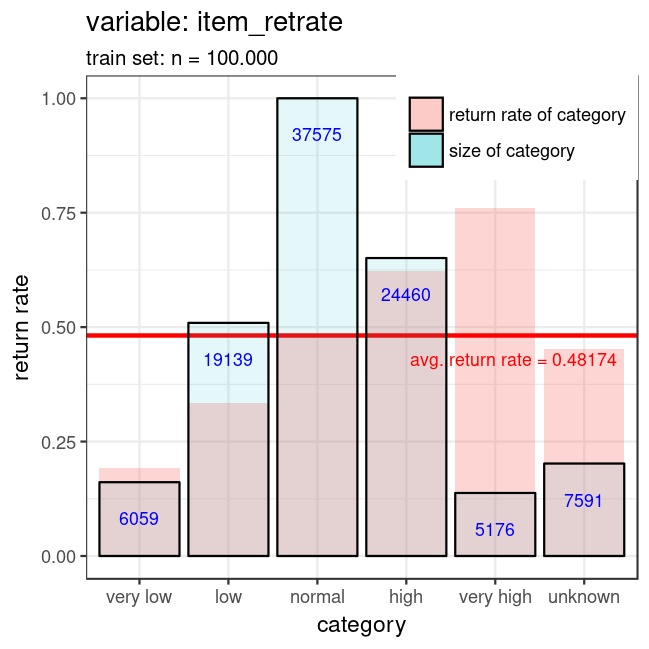
\includegraphics[width=0.5\textwidth]{pictures/item_retrate_r.png}}
	\subfigure[]{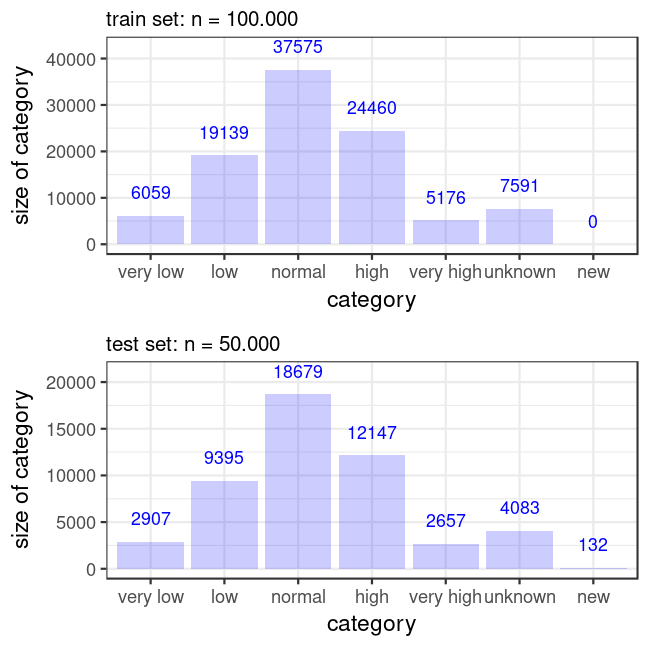
\includegraphics[width=0.5\textwidth]{pictures/item_retrate_ku.png}}
	\caption{(a) Display of the artificially created feature \texttt{item\_retrate}. red shading: average return rate of observations of this category with comparison to average return rate of all items in training set (red line, avg.returnrate = 0.48174). blue histogram: number of observations in each category. (b) Distribution of variable \texttt{item\_retrate} in train and test set. In both data sets the newly created variable follows a similar distribution.}
	\label{Figure::ItemRetrate}
\end{figure}

 \begin{figure}
  \begin{minipage}[c]{0.65\textwidth}
    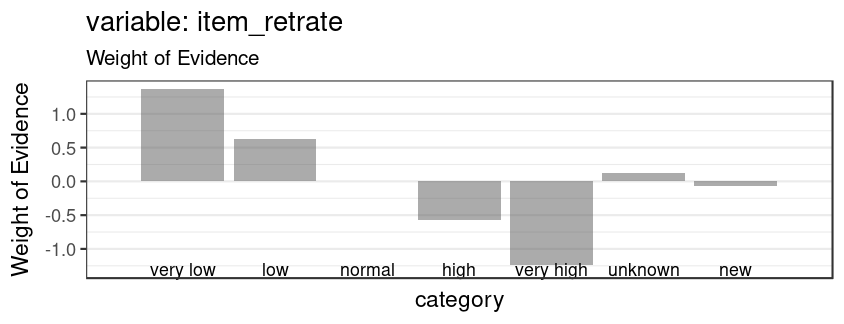
\includegraphics[width=\textwidth]{pictures/item_retrate_woe.png}
  \end{minipage}\hfill
  \begin{minipage}[c]{0.35\textwidth}
    \caption{Weight of Evidence (WOE) of the feature \texttt{item\_retrate}. Categories "very low" to "very high" were created by grouping the items  according to their return rate in the training set. This created a strong feature in terms of WOE.} \label{Figure::ItemRetrateWOE}
  \end{minipage}
\end{figure}

\subsection{item\_type}
High cardinality attributes are impractical for most predictive algorithms. The original data set contained the variable \texttt{item\_size}, which overall consists of more than 100 categories. Even after merging duplicate naming such as (... xs, s, m, l, ...) and (... XS, S, M, L, ...), the variable is still of high cardinality. One method of reducing the categories of a variable is semantic grouping (c.f. \cite{moeyersoms2015}). Categories were generated with respect to common sizing systems for shoes and clothes. Additionally the category \texttt{rest} stores items that could not be allocated to shoes or clothes and \texttt{unsized} stores items without a specific size. By using semantic grouping it was not only possible to reduce over 100 categories to only four, but also a difference in the return rate of the categories can be observed. Figure \ref{Figure::ItemType} shows that \texttt{unsized} has a considerably lower return rate than average (Also the return rate of \texttt{rest} is lower than average, but because of the small size of the category it will not add much information to the model.)

\begin{lstlisting}
shoes = c(30:48, paste(35:46, "+", sep = ""),
          1:9, paste(1:12, "+", sep = ""))
clothes = c("xs", "s", "m", "l", "xl", "xxl", "xxxl",
            "XS", "S", "M", "L", "XL", "XXL", "XXXL",
            100:176)
unsized = c("unsized")

item$type                               = "rest"
item$type[item$item_size %in% shoes]    = "shoes"
item$type[item$item_size %in% clothes]  = "clothes"
item$type[item$item_size %in% unsized]  = "unsized"

\end{lstlisting}

\begin{figure}
  \begin{minipage}[c]{0.55\textwidth}
    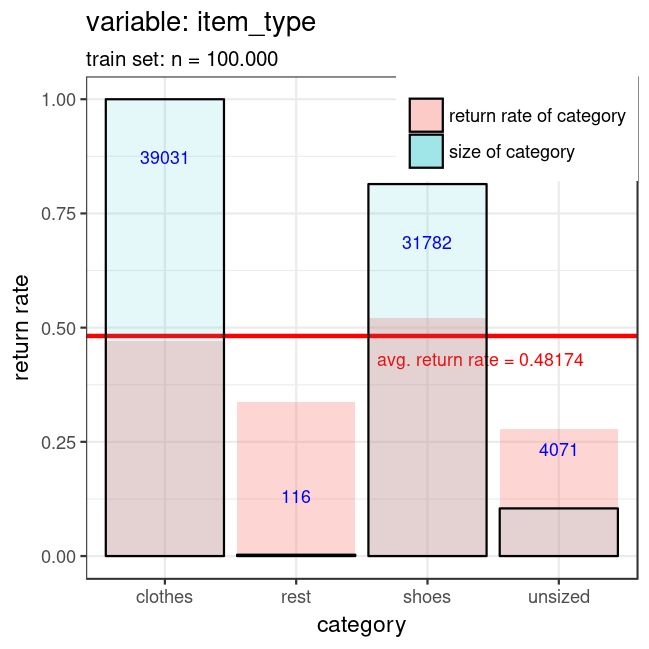
\includegraphics[width=\textwidth]{pictures/item_type.png}
  \end{minipage}\hfill
  \begin{minipage}[c]{0.4\textwidth}
    \caption{Display of the artificially created feature \texttt{item\_type}. red shading: average return rate of orders in this categories in training set. blue histogram: number of orders of each category.}
    \label{Figure::ItemType}
  \end{minipage}
\end{figure}



\section{Preparation of Data Set for Models}

\subsection{Decomposition due to uncertain categories}\label{Subsec::4Split}
When creating the variables \texttt{item\_retrate} and \texttt{user\_retrate} (section \ref{Subsec::ItemRetrate}), it is only justified to infer from items/user that occur more than 15/6 times (explanation see \ref{Subsec::Interval}). All remaining items/user were stored in the category \texttt{unknown}. However, this category can not be treated like the categories "very low" to "very high" that are directly connected to the previous return rate of the item/user. To ensure that the predictive algorithm does not treat the category incorrectly, the data set gets decomposed into certain and uncertain subsets, as shown in Table \ref{Figure::Decomposition}. The decomposition ensures that in each subset the remaining columns are "pure" (do not contain category \texttt{unknown} or \texttt{new}). For example subset \texttt{.u} (second row) is the subset, where the column \texttt{user\_retrate} got removed and \texttt{item\_retrate} contains only certain categories. 
\begin{lstlisting}
# .u       : model without user_retrate
# remove   : "unknown" and "new" of "item_retrate"
# model    : item_retrate is clean now, can be used for model
known.u    <- known[item_retrate!="unknown" & user_retrate=="unknown",]
unknown.u  <- unknown[item_retrate!="unknown" & item_retrate!="new",]
unknown.u  <- unknown.u[user_retrate=="unknown" | user_retrate=="new",]
\end{lstlisting}
Therefore the model is trained on this subset without the feature \texttt{user\_retrate} and accordingly predicts the \texttt{unknown.u} subset. Actually for training the model not only the \texttt{known.u} subset can be used, but also the \texttt{known.f} subset, since it is only important that the remaining columns are pure.\\
\begin{center}
\begin{figure}[h]
\begin{tabular}{|c | c| c || r | r|}
\hline
\textbf{user\_retrate} & \textbf{item\_retrate} & \textbf{rest} & \textbf{model} & \textbf{size (train/test)}\\
\hline \hline
1 & 1 & 1 & .f - full model & 25266 / 10082\\
\hline
u/n & 1 & 1 & .u - without user\_retrate & 67143 / 35703\\
\hline
1 & u/n & 1 & .i - without item\_retrate & 1857 / 813\\
\hline
u/n & u/n & 1 & .iu - without item\_retrate & 5734 / 3402\\
& & & and user\_retrate & \\
\hline
\end{tabular}
\captionof{table}{Decomposition of data set due to uncertain categories. u/n stands for "unknown" and "new" categories (= uncertain categories), 1 for certain categories. Categories "unknown" and "new" in item\_retrate and user\_retrate are uncertain and should not be included in models. Decomposition in pure subsets ensures that model only is fed with certain categories.}
\label{Figure::Decomposition}
\end{figure}
\end{center}
\newpage
In total four models get trained and used for prediction (full model, without item\_retrate, without user\_retrate, without item\_retrate and user\_retrate). This decomposition increased the performance from $loss_{full} = -243104.7 $ and $AUC_{full} = 65.27\%$ to $loss_{dec} = -239499.7 $ and $AUC_{dec} = 66.52\%$ (with a tuned neural network).

\subsection{On multiple $\tau$ thresholds}\label{Subsec::Tau}

By observing the given loss table for this specific task (see Table \ref{cost matrix}), it is evident that depending on item price, type 1 errors can be more penalising than type 2 errors and vice versa.
In order  to optimise the results, an analysis of its explicit dependence from item\_price is due.
\newline
The essential boundaries of when type 1 and type 2 errors are equally relevant are to be assessed, resulting in a meaningful first split of the data. In most cases $\tau<0.5$ and $\tau>0.5$ are found to be optimal when type 2 error loss is bigger and smaller than type 1 error loss respectively.
  \newline
 For this particular case study only one boundary is to be found because it is the root of a grade 1 polinomial 
 \begin{eqnarray}
 \Delta:=-0.5 \cdot 5(3+0.1 \cdot X)+0.5 \cdot X
 \label{boobies}
 \end{eqnarray}
 
To decrease the loss even further, a split of the train and test sets depending on item\_price is a natural extension of this first remarks.
The difference of type 2 and type 1 error magnitudes $\Delta$ is a linear function of item\_price so a split in a quantile\-like way is recommended, but with one of the boundaries being $30$ euros (see equation \ref{boobies}).
\begin{center}
\begin{table}[h]
\begin{tabular}{|l|| c | c | c | c | c | c |}
\hline
\textbf{tau category} & 1 & 2 & 3 & 4 & 5 & 6 \\
\textbf{item\_price}  & {[}0,30)   & {[}30,59)   & {[}59,79)  & {[}79,90)   & {[}90,120)    & {[}120, max(item\_price){]} \\
\hline
\end{tabular}
 \caption{Definition of tau categories. Every order is sorted to an tau category, depending on the price of the item that got ordered.}
 \label{Table::Tau}
\end{table}
\end{center}
Implementing this dependence in the cross validation code is essential not only to be able to estimate accuracy through AUC (and other measures) and tune parameters , but also to obtain an estimate of the specific total loss of a prediction.\\
Running the cross validation for each of $$T_k:=\{observation \in Split.Train \ | \ \tau = k\}$$ produces significantly different optimal values for $\tau$ (see Table \ref{Table::Moobs}), which is a confirmation of what was expected from the above reasoning. 

%------------------------------------------------------------
\section{Cross Validation - Theory}

Let's assume to be in one of the following situations: 
\begin{itemize}
\item the prediction algorithm of choice has a variety of parameters that need to be tuned, which means optimised in order to improve accuracy (or any other measure of goodness)
\item performances of a group of completely different models need to be assessed and ranked for selection purposes
\end{itemize}
Cross validation is a widely (if not the most) used class of methods to assign to each different model an estimate of their "goodness". A great asset of cross validation is that it offers the flexibility to choose the most appropriate measure of goodness, depending on the situation. Such measures can be the very intuitive accuracy, the ever popular AUC or, as in this paper's case study, a customised function depending on a loss matrix (in this case Table \ref{cost matrix}).\\
The class of Cross Validation (CV) methods contains, among others:
\begin{itemize}
\item K-fold CV
\item leave-one-out CV (limit case of K-fold for $K:= \# \{ training \enskip set\}$)
\item stratified K-fold CV
\item N-repeated stratified K-fold CV
%\item Monte Carlo C.V.
%\item Generalised CV
\end{itemize}
The method that was chosen for this study is a 6-repeated  stratified 3-fold CV, which offers a good balance between accuracy and computational intensity. 

\subsection{N-repeated stratified K-fold C.V.}

Suppose a training set $T$ is given so that every $(v_{i}, y_{i}) \in T$ is of the form $(v_{1,i}, .., v_{u,i}, y_{1,i}, .., y_{v,i})$ where $u$ is the number of explanatory variables, $v$ is the number of outcomes.

\begin{definition}
A subset $T_{k} \subset T$ is called a stratified K-fold of $T$ if 
\begin{enumerate}
\item their cardinalities follow relation $$ \# T_{k} = \Big\lfloor \frac{\#T}{K} \Big\rfloor $$
\item is picked randomly from the family of subsets of $T$ such that $$ \mathbb{E}_{T_{k}} [y] = \mathbb{E}_{T} [y]$$
\end{enumerate}
\end{definition}

First of all $\forall k \in 1, ..,K$ a stratified K-fold $T_{k}$ of $T$ is taken. A model prediction will be called $ \hat{M}(\cdot,\theta)$ for simplicity and in order to stress its dependence from the parameter $\theta$ to be tuned.
Note that $\hat{M}(\cdot,\theta)$ could be interpreted as a total different model prediction $\hat{M}_{\theta}$ as well.\\
The second step consists in training the model on $T \setminus T_{k} \enskip \forall \theta_{i} \in \Theta $ the parameter candidates set (from now on we use the simplified notation $ \hat{M}_{k}(\cdot,\theta):=\hat{M}_{T \setminus T_{k}}(\cdot,\theta)$ ).
Finally $\forall (v_{j},y_{j} \in T_{k} $  $$ L(\hat{M}_{k}(v_{j},\theta_{i}),y_{j})$$ is calculated and the results summarised in the following way (C.f. \cite{tibshirani2009} ) $$ CV(\theta):= \frac{1}{\#T} \sum_{k=1}^{K} \sum_{j \in C_{k}} L(\hat{M}_{k}(v_{j},\theta),y_{j})$$
For minimisation and maximisation reasons the multiplication by $\frac{1}{\# T}$ is irrelevant so it can be omitted.

%------------------------------------------------------------
\section{Cross Validation - Implementation}


Script \texttt{00-1-kfold.R} performs k-fold cross validations for n variations of settings for a neural network. In order to perform a k-fold cross validation, the dataset is randomly split into k subsets folds(line 5). For every run i of the k-fold cross validation subset \texttt{folds==i} is left out for prediction, which means that the model is trained on the subset without \texttt{folds==i} and the prediction is performed on subset \texttt{fold==i}. This split is performed in lines 17-22, followed by training the model (line 24) and prediction (line 29). Note that the second @@@@laufindex n indicates the settings for the neural network (line 27+28). This index n is changed by the outer foreach-loop (line 11). \\
To evaluate the performance of the model, the loss \ref{@@@} is used as a measure (line 30). \\
\\
In order to decrease run time, the script uses the package \texttt{"doParallel"} for parallel computing. Lines 7-9 define the settings for parallel computing. In line 14 the nesting operator \texttt{\%dopar\%} starts parallel computing, so that different runs of the foreach-loop can be performed by a different cores at the same time.\\ 
The output of the k-fold cross validation is a k*n matrix (k: k-fold cross validation, n: number of variations of settings for model), where every element consists of a list  of the measure and the settings of the model (line 36). \\

\begin{lstlisting}[language=r]
# 00-1-kfold_cv.R
k = k              # dimension of cv is choosen in parent script
sample.idx = sample(nrow(tr.v))
train.rnd  = tr.v[sample.idx,] 
folds      = cut(1:nrow(train.rnd), breaks = k, labels = FALSE)
# settings for parallel computing
nrOfCores = detectCores()
cl        = makeCluster( max(1,detectCores()-1))
registerDoParallel(cl)
# loops for cross validation and tuning
results.par = foreach(n = 1:nrow(parameters), .combine = cbind, 
                      .packages = c("caret", "nnet", "data.table")) %:%
    foreach(i = 1:k, 
            .packages = c("caret","nnet", "data.table")) %dopar%{
        set.seed(1234) # set seed for reproducibility 
        # Split data into training and validation
        idx.val  = which(folds == i, arr.ind = TRUE)
        cv.train = train.rnd[-idx.val,]
        cv.train = cv.train[order(cv.train$order_item_id),]
        cv.val   = train.rnd[idx.val,]
        cv.val   = cv.val[order(cv.val$order_item_id),]
        price    = real_price$item_price[cv.val$order_item_id]
        # train nnet and make prediction
        nnet     = nnet(return~. -order_item_id - tau, 
                        data  = cv.train,
                        trace = FALSE, maxit = 1000,
                        size  = parameters$size[n], 
                        decay = parameters$decay[n])
        yhat.val = predict(nnet, newdata = cv.val, type = "raw")
        loss     = helper.loss(tau_candidates = tau_candidates, 
                               truevals       = cv.val$return, 
                               predictedvals  = yhat.val, 
                               itemprice      = price)
        pars     = data.table("size"  = parameters$size[n],
                              "decay" = parameters$decay[n])
        res      = list("loss"        = max(loss), 
                        "parameters"  = pars)
        }
stopCluster(cl) # stop parallel computing

\end{lstlisting}

Since the performance of the model also depends on the 'quality' of the training data and the training data is determined randomly, it is crucial to change the randomness of the splits. By varying the seed \texttt{set.seed(1234*t)} in the mother script  \texttt{00-2-rep\_cv.R} , the randomness of the training set tr is changed (line 11-16). \\ 
Further this script \texttt{00-2-rep\_cv.R} splits the dataset according to the six tau-categories (see Table \ref{Table::Tau}). The k-fold cross validation from the previous section is then performed for every of these subsets. The results for each tau-category \texttt{v} are then stored in a list \texttt{tau\_c} (line 22). \\
The output of the m-times repeated cross validation is a list of m times the same cross validation procedure (only with different randomness). Each element of the m-sized list is a list of the k*n matrix for the six tau-categories v.\\
(m : number of repeated cross validations (same procedure but different randomness), v : six tau-categories, k : k-fold cross validation, n : number of variations of settings for model)\\ 

\begin{lstlisting}
tau_c   = list()
cv.list = list()

for (t in 1:m){
    set.seed(1234*t)
    # Splitting the data into a test and a training set 
    idx.train = caret::createDataPartition(y = known$return, p = 0.8, list = FALSE)
    # Actual data splitting
    tr = known[idx.train,  ] # training set
    ts = known[-idx.train, ] # test set
    for (v in 1:6){
        # call script for each tau-class
        tr.v = tr[tr$tau == v, ]
        print(paste("tau =", v, "rep = ", t))
        source(file = "./nnet/00-1-kfold_cv.R")
        tau_c[[paste("tau_c ==", v)]] = results.par
  }
  cv.list[[t]] = tau_c
}
\end{lstlisting}



Section \ref{Subsec::4Split} explains the importance of decomposing our dataset into four subsets according to the explanatory power of the features for training. In script \texttt{01-par-tuning.R} the whole tuning-process is performed for the different subsets. The following explains the preparation of the .u subset exemplarily.\\
The known dataset consists of the subsets where a full model can be trained (.f) and the subset where the model without \texttt{user\_retrate} can be trained (\texttt{.u}). These two subsets are combined to the known data set (line 51). For training a neural network additional data preparation as described in section \ref{Subsec::AddPrep} is necessary (line 54). Then the columns of the feature \texttt{user\_retrate} get removed and the set is named according to the requirements of the script for cross validation (lines 55-59). \\
After performing the m times repeated k-fold cross validation for the n variations of settings for the model, the results are stored in a the list \texttt{cv.list.u} for further evaluation (line 71).

\begin{lstlisting}[language=r]
known   = rbind(known.f, known.u) # can also use .f for training, variables are pure
unknown = unknown.u               #
# additional data preparation for nnet
source(file = "./nnet/00-3-nnet_DataPrep.R")
known.n$user_retrate   = NULL     # remove user_retrate (uncertain categories)
unknown.n$user_retrate = NULL     #
                                  #
known   = known.n                 # output of additional data preparation
unknown = unknown.n               #

# perform repeatet cross validation
source(file = "./nnet/00-2-rep_cv.R")
cv.list.u   = cv.list             # store result of repeated cross validation

\end{lstlisting}


%----------------------------------------------------------------

\section{Classification Alogrithms}

\subsection{Extreme Gradient Boosting}
Extreme Gradient Boosting is a gradient boosting decision tree algorithm. Boosting refers to an additive training technique where starting with some base classifiers $\hat{y}^{(0)}= f_0(x_0)$, an objective function $F(y,f_k)$,

\begin{eqnarray*}
F = \displaystyle\sum_{i=1}^{N} l(y_i, \hat{y}_i) + \displaystyle\sum_{k=1}^{K} \Omega(f_k) 
\end{eqnarray*}

that consists of a training loss term $l(y_i,\hat{y}_i)$ and a regularization term $\Omega(f_k)$ gets optimized by adding at each iterative stage a term to the classifier function that compensates for the errors of the previous model. 

\begin{eqnarray*}
\hat{y}^{(0)} &=& 0       \\
\hat{y}^{(1)} &=& \hat{y}^{(0)} + f_1(x_1) =  f_1(x_1)   \\
\hat{y}^{(2)} &=& \hat{y}^{(1)}+f_2(x_2) = f_1(x_1) + f_2(x_2) \\
&\vdots& \\
\hat{y}^{(t)} &=& \displaystyle\sum_{k=1}^{K} f_k(x_k) = \hat{y}^{(t-1)} + f_t(x_t)
\end{eqnarray*}

This sequential procedure stops when no further improvements can be made, e.g. when the reduction of the loss term is smaller then the change in the regularization term. \\

%--------------------------------------------------------
\subsection{Random Forest}
A random forest is an ensemble of tree classifiers with implemented randomisation procedures.
Random forest tends to be good out of the box and apt for parallelization.

\begin{definition}
A tree-structured classifier $h_{\theta_{k} }(\textbf{x})$ is a generalised step function $h_{\theta_{k} }: \textbf{X} \rightarrow F \subset \mathbb{R}$ where $\textbf{X}$ is the data set and $F$ is a finite cardinality set. This function has constant values on a partition of the data set consisting of hyper-rectangles.
\end{definition}
Note that $\theta_{k}$ indicates how to create such a partition by determining 
\begin{enumerate}
\item predictors to split on
\item values of the splits
\item depth of the tree
\end{enumerate}
where the first is a randomly chosen subset of the parameters of cardinality equal to \textit{m\_tree} in the \textit{random.Forest} package, the second is chosen in order to maximize information gain, the third corresponds to \textit{n\_tree} in \textit{random.Forest}. 

The concept of generalization error for a random forest was first presented in \cite{breiman2001random}. The following theory represents the theory introduced in the article. 

\begin{definition}
A random forest is a classifier consisting of a collection of tree-structured classifiers $\{h( \textbf{x},  \theta_{k} ) \mid k \in  \overline{n} \}$ where the $\theta_{k}$ are i.i.d. random vectors and each tree casts a unit vote for the most popular class at input $\textbf{x}$.
\end{definition}

For notation simplicity purposes, from now on, $h( \textbf{x},  \theta_{k} )$ can be replaced with $h _{k}( \textbf{x} )$ and viceversa.
\begin{definition}
Given $\{h_{k} ( \textbf{x}) \mid k \in  \overline{K} \}$, the training set drawn
at random from the distribution $\textbf{X}$ and its realisation $Y$ (through $h(\cdot)$), define the margin function as $$mg(\textbf{X},Y)= \sum_{k=1}^{K} \frac{I(h_{k}(\textbf{X})=Y) }{K} - \max_{j \neq Y}  \sum_{k=1}^{K}\frac{I(h_{k}(\textbf{X})=j) }{K} $$
where $I (\cdot)$ is the indicator function. 
\end{definition}
The margin measures the extent to which the average number of votes at $\textbf{X}, Y$ for the right class exceeds the average vote for any other class. The larger the margin, the more confidence in the classification. \\
The generalization error is given by
$$\mathbb{P}(mg(\textbf{X}, Y)<0)$$
where the probability is over the $(\textbf{X}, Y)$ space.
For a large number of trees, it follows from the
Strong Law of Large Numbers and the tree structure that:
\begin{theorem}
As the number of trees $K$ increases, the generalization error converges almost surely to
$$\mathbb{P}_{\textbf{X}, Y}(\mathbb{P}_{\theta}(h(\textbf{X}, \theta) = Y)- \max_{j \neq Y} \mathbb{P}_{\theta}(h(\textbf{X}, \theta) = j) < 0)$$
which assures the method does not overfit for big ensembles of trees.
\end{theorem}

\begin{proof}
By definition of almost sure convergence, it suffices to show that there is a set of probability zero $C$ on the sequence space  $\{\theta_{k} \mid k \in K \}$ such that outside of $C$, $\forall x$,
$$ \sum_{k=1}^{K} \frac{I(h(\textbf{x},\theta_{k})= j) }{K} \rightarrow \mathbb{P}_{\theta}(h(\textbf{x}, \theta) = j)$$
For a fixed training set and fixed $\theta$ , $\{x \mid h(x, \theta) = j \}$ is a union of hyper-rectangles. This follows from the definition of decision tree. Moreover, $\forall$  $h(x, \theta)$ $\exists !$ $ T < \infty$ number of such unions of hyper-rectangles, denoted by $S_{1},..., S_{T}$ . Define $\phi(\theta) = t$ iff $\{x \mid  h(x, \theta) = j \} = S_{t}$. Let $K_{t}$ be the number of times that $\phi(\theta_{k}) = t$ in the first $K$ trials. Then
$$ \sum_{k=1}^{K} \frac{I(h(\textbf{x},\theta_{k})= j) }{K} = \sum_{t} \frac{K_{t}I(x \in S_{t}) }{K}$$
By the Law of Large Numbers,
$$K_{t} = \sum_{k=1}^{K} \frac{I(\phi(\theta_{k})= t) }{K} $$
converges almost surely to $\mathbb{P}_{\theta}(\phi(\theta) = t)$. Taking unions of all the sets on which convergence does not occur for some value of $k$ gives a set $C$ of zero probability such that outside of $C$,
$$ \sum_{k=1}^{K} \frac{I(h(\textbf{x},\theta_{k})= j) }{K} \rightarrow \sum_{t} \mathbb{P}_{\theta}(\phi(\theta) = t)I(x \in S_{t})$$
The right hand side is $\mathbb{P}_{\theta}(h(\textbf{x}, \theta) = j)$ ✷
\end{proof}

The model default parameters are (c.f. \cite{breiman2001random})
\begin{enumerate}
\item m\_tree:  $(\#features) \cdot \frac{1}{3} $ for regression, $ (\#features)^{1/2}$ for classification
\item n\_tree:  $500$
\item nodesize: $1$ (for classification), $5$ (for regression)
\end{enumerate}
%----------------------------------------------------------

\subsection{Neural Network}

Neural networks were first developed in the middle of the twentieth century, had great importance for a few decades and then overshadowed by other algorithms such as support vector machines in the later decades of the last century until they were discovered to be great in performance when paired with backpropagation for unsupervised learning.
The idea behind this category of algorithms is that most real life problems are highly non linear, and therefore standard models such as linear regression will not be suited for approximation of reality.
\begin{figure}
  \begin{minipage}[c]{0.65\textwidth}
    \includegraphics[width=\textwidth]{pictures/nnet_1.png}
  \end{minipage}\hfill
  \begin{minipage}[c]{0.35\textwidth}
    \caption{An example of a neural network structure map. In this particular case there are three input variables, two hidden layers consisting of four and three neurons respectively and two output variables.
    Note that in the \textit{nnet} R-package there is only one hidden layer. Source: \cite{lecun2015}}
    \label{Figure::Nnet_1}
  \end{minipage}
\end{figure}
The way this class of algorithms work is calculating numerous weighted linear combinations of the input variables and applying a non linear function to it.
This procedure is repeated multiple times depending on the design of the network, each of these basic operation is called a neuron.
The group of neurons on a same level is called hidden layer, there can be multiple hidden layers each performed taking the outputs of the previous one (altough the \textit{nnet} package uses only one, see Figure \ref{Figure::Nnet_1}).
Neural networks not only depend on the number of neurons for each hidden layer (this is called \textit{size} in \textit{nnet} package), number of layers and definition of input variables for each neuron. In fact they are defined also by which nonlinear function is applied in each neuron: the traditionally used are sigmoid functions such as hyperbolic tangent and logistic function, $$f_{1}(t):=\tanh(t) \quad f_{2}(t):= \frac{1}{1+ e^{-t}} $$ the latter being used in the \textit{nnet} package. The reason for the application of such functions for each elementary step is an attempt to linearise the boundary of highly nonlinear sets. 
\subsubsection{Backpropagation}
Backpropagation is one of the milestones of the development of neural networks and plays a fundamental role especially for deep networks, which consist of multiple hidden layers.
This process aims to find out the most appropriate weights $w_{i,j}$ for the construction of each neuron in the net (see Figure \ref{Figure::Nnet_1}).
To start with an objective function, generally a loss function, is differentiated and used as in Figure \ref{Figure::Nnet_2} together with the chain rule to find partial derivatives of the error function with respect to the weights $w_{i,j}$ for each stage and using gradient descent method with learning rate $\eta$ (which is often associated with the parameter \textit{decay} in \textit{nnet}) to define new weights $$\hat{w}_{i,j}:=w_{i,j}- \eta \frac{\partial E}{\partial w_{i,j}}$$
One might think that local minima might be a problem, luckily \textit{"Regardless of the initial conditions, the system nearly always reaches solutions of very similar quality. Recent theoretical and empirical results strongly suggest that local minima are not a serious issue in general."} (C.f. \cite{lecun2015}).
Once the weights and structure of the network are determined it is a mere substitution that will produce the results for each different input.
\begin{figure}
  \begin{minipage}[c]{0.65\textwidth}
    \includegraphics[width=\textwidth]{pictures/nnet_2.png}
  \end{minipage}\hfill
  \begin{minipage}[c]{0.35\textwidth}
    \caption{Diagram on how the backpropagation procedure is carried out. Starting from the error $y_{l}-t_{l}$, the chain rule of derivatives is used to explicit a variation in the error as function of variations in the input variables. Note that the error is taken as the differentiation of a loss function: in this case $\frac{1}{2} (y_{l}-t_{l})^{2}$. Source: \cite{lecun2015}}
    \label{Figure::Nnet_2}
  \end{minipage}
\end{figure}
%--------------------------------------------------------

\subsubsection{Additional Data Preparation}\label{Subsec::AddPrep}
The performance of neural networks increases, when the data is numerical (instead of categorical). Different techniques can be used to convert a categorical variable to a numerical, but not every technique is suitable for every case.\\
Since item\_retrate and user\_retrate are based on their connection to the target variable, assigning the Weight of Evidence (WOE) to each category does not aggravate overfitting even more. The WOE is also used for the categories of delivery\_time and price\_comp, but to prevent overfitting, the WOE was calculated on a small subset of the train set, that is not going to be used for training anymore (c.f.\cite{moeyersoms2015}):\\
If the variable only has few categories, it is beneficial to introduce dummy variables. Instead of having one variable item\_type with four categories, there will be four binary dummy variables that indicate whether the item is of this category. 
\\
The advantage of dummy variables is, that they are independent of the target variable but since every category requires a new dummy variable, they should only be used for lower dimensional variables (c.f. \cite{moeyersoms2015}).

\section{Parameter Tuning}

\subsection{Parameters of Neural Network}\label{Subsec::ParsNNet}
To increase the performance of a model it is vital to use the optimal parameter depending on the input data. Since the data set is decomposed into four subsets, that differ in the composition of predictive variables (see section \ref{Subsec::4Split}), the tuning needs to be performed on every subset separately. In the following the subset test.u (model without the variable user\_retrate) is evaluated exemplarily.\\
The results of the parameter tuning are shown in Figure \ref{Figure::ParameterGraph}. The data set was divided into six subsets according to their tau-categories (see section \ref{Subsec::Tau}). The tuning parameters are as follows: size of the hidden layer: [3, 5, 7, 9, 11, 13, 15] and decay: [0.01, 0.1, 0.5, 0.8, 1.0].\\
\begin{center}
\begin{tabular}{| l || c | c | c | c | c |}
 \hline
 \textbf{index}  & 1 - 7 & 8 - 14 & 15 - 21 & 22 - 28 & 29 - 35\\
 \hline
  \textbf{decay} & 0.01   & 0.1     & 0.5     & 0.8   & 1.0 \\
  \hline
 \textbf{size}   & 3, 5, 7, 9, & 3, 5, 7, 9, & 3, 5, 7, 9, & 3, 5, 7, 9, & 3, 5, 7, 9,\\ 
                 & 11, 13, 15  & 11, 13, 15  & 11, 13, 15  & 11, 13, 15  & 11, 13, 15 \\
\hline 
%\caption{Explanation}
\end{tabular} 
\end{center} 
\vspace{0.8cm}

Figure \ref{Figure::ParameterGraph} shows that for every tau-category the loss is more stable for larger decay values. For higher decay values, the size of the hidden layer has only marginal influence on the loss. Hence it is not necessary to find the exact optimal parameter for every tau-category and train a separate model on this category (within a certain range of parameters). Further it is even beneficial to refrain from splitting into tau-categories, and instead training only one model with almost optimal parameters on the whole dataset. Then the training data carries sixfold as many observations which enables a better training of the neural network.\\
The sum of the six normed tuning graphs of Figure \ref{Figure::ParameterGraph} is shown in Figure \ref{Figure::NormedSum}. The almost optimal parameters are extracted from the maximum of the loss. (index 25 $\rightarrow$ size of hidden layer: 9, decay: 0.8).\\
In order to increase the reliability of the tuning results, they were calculated of a 3-fold cross validation, that got repeated 6 times (ensuring that the datasets are sampled differently). 

\begin{figure}
 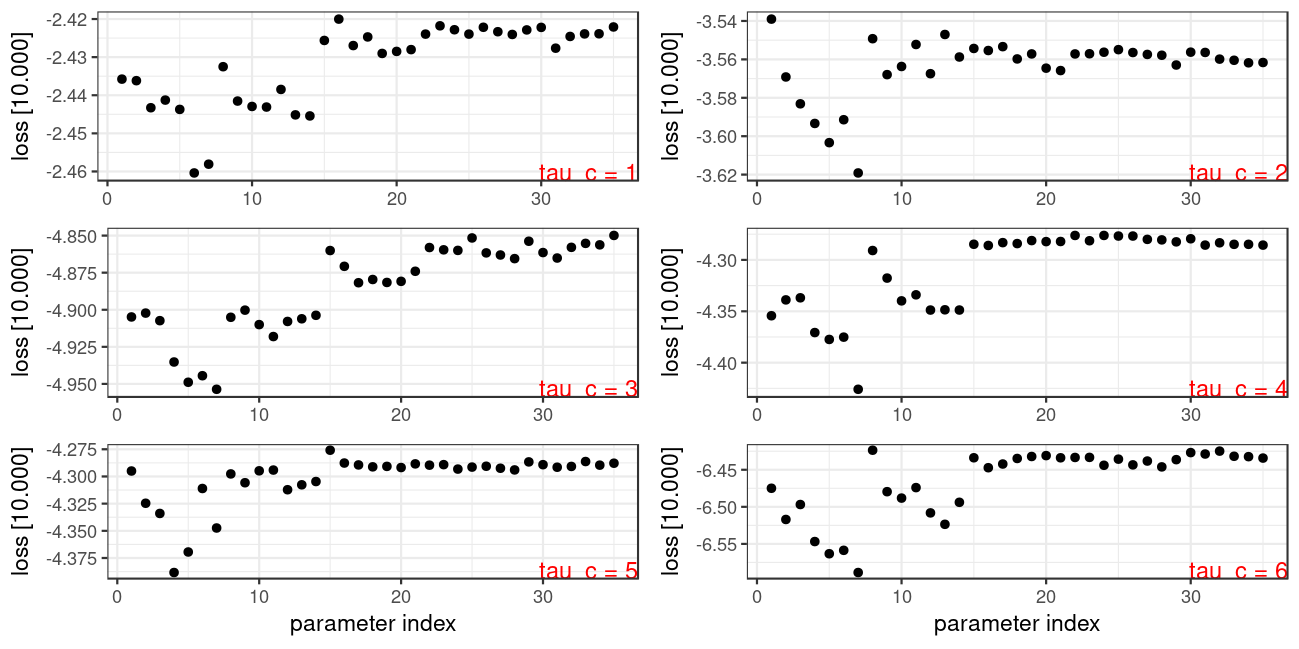
\includegraphics[width=\textwidth]{pictures/nnet_tuning.png}
 \caption{Tuning graph for the six different subsets (according to tau categories). For every subset 35 different models were trained and the loss of each prediction calculated. The settings change as follows: size = 3, 5, ... , 15 then dacay = 0.01, 0.1, 0.5, 0.8, 1.0. Stable loss values for bigger decays, size does not have much influence for high decay values.}
 \label{Figure::ParameterGraph}
\end{figure}

\begin{figure}
  \begin{minipage}[c]{0.65\textwidth}
    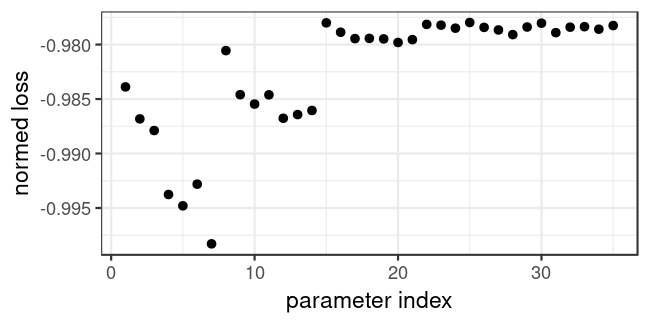
\includegraphics[width=\textwidth]{pictures/normed_sum.png}
  \end{minipage}\hfill
  \begin{minipage}[c]{0.35\textwidth}
    \caption{Sum of normed tuning graphs of the six subsets from graph \ref{Figure::ParameterGraph}. Loss is the highest for bigger decay values. Size only has little influence on loss values for high decay values.}
    \label{Figure::NormedSum}
  \end{minipage}
\end{figure}


\subsubsection{optimal $\tau$ for loss function}
With the parameters from the previous section (\ref{Subsec::ParsNNet}), the neural network has optimal performance for our needs. As a last step the threshold value $\tau$ (which is the threshold that decides if the predicted probability is big enough to be assigned as 1 (item is returned) or stays 0 (item is not returned)) needs to be tuned to minimize the loss function. As described in section \ref{Subsec::Tau}, the loss depends on the item price and therefore the data set is split into six subset according to the price (subsets are called tau-categories). \\
Figure \ref{Figure::FindTau} displays the loss function for the six tau-categories. In each category the loss is calculated for each possible $\tau$ value. The function reaches its maximum in the range between $\tau=0.45$ and $\tau = 0.65$, depending on the category. The maximum of the function is the optimal $\tau$ that minimizes the loss of the subset. It is not surprising that for categories 1 to 6 (where 1 are cheapest and 6 most expensive items (see \ref{Subsec::Tau})) the optimal $\tau$ increases. (Interpretation of $\tau$ in connection to item price and return probability in section \ref{Subsec::Tau}.)

\begin{figure}
 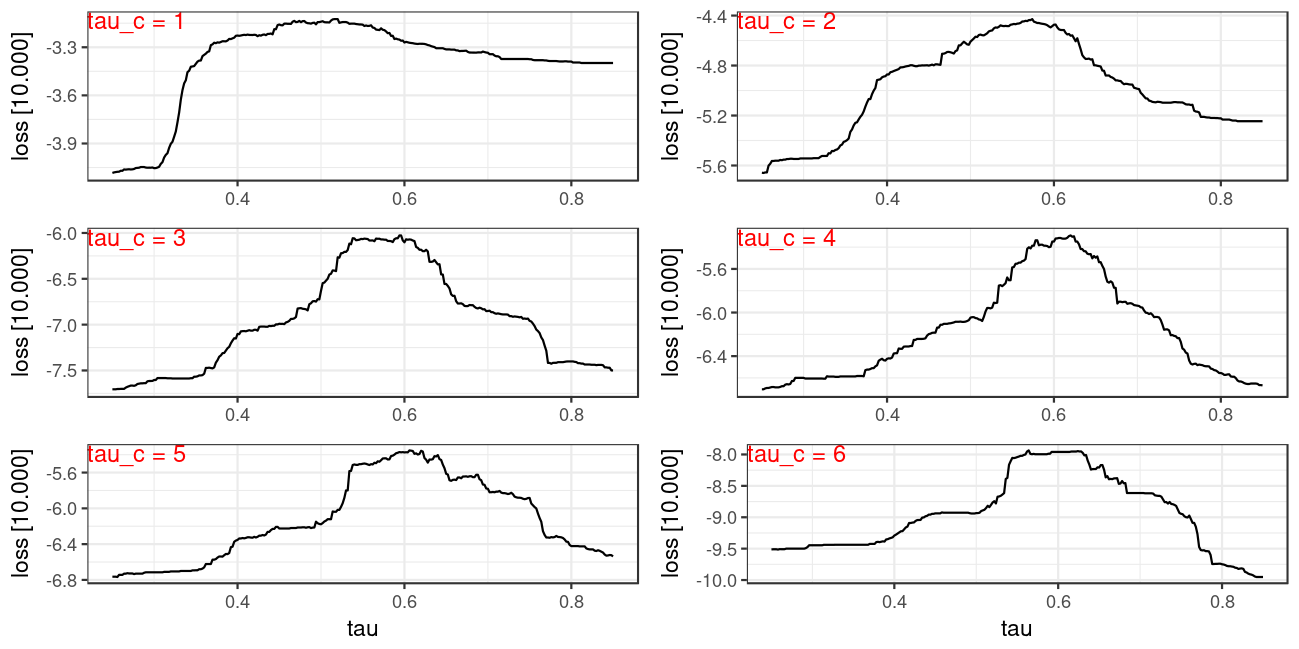
\includegraphics[width=\textwidth]{pictures/find_tau.png}
 \caption{Loss function for the six tau-categories. In each category the loss is calculated for each tau-candidate. The negative loss shows its maximum in the range between $\tau=0.45$ and $\tau = 0.65$.}
 \label{Figure::FindTau}
\end{figure}

\subsection{Performance Benchmark}

The following table shows how neural network outperformed random forest and xgboost in this problem for a set of 25000 observations. Double values are expected in the test set, which contains 50000 observations.

\begin{table}[h]
\centering
\label{my-label}
\begin{tabular}{|lc|}
\hline
\textbf{Prediction} & \textbf{Estimated total loss} \\
\hline \hline
trivial 1 (vector consisting of ones only)                         &  $- 415415.6   $            \\
trivial 0 (vector consisting of zeros only)                       & $- 321240.2 $            \\
random 01 vector with $mean=0.48$                            &  $- 365703.9  $                \\
\hline
first randomForest ($\tau=0.5$)                                     & $- 321420.5$                \\
tuned randomForest (optimised multiple $\tau$)          &  $-260608.5$               \\
tuned xgboost (optimised multiple $\tau$)         & $-290419.9$ \\
tuned nnet (optimised multiple $\tau$)                          & $-239499.7$                   \\
\hline
\end{tabular}
\caption{Estimated total loss of random forest, xgboost and nnet in comparison to trivial predictions. Performed on 25000 observations (25\% of train set.}
\end{table}

\subsection{Prediction}
In order to construct values for a comparison of the performance on the test dataset, the prediction is run on the training dataset. Therefor the training dataset is randomly split into a new training and test dataset. After training and predicting with the four models (.f, .u, .i and .iu), the loss is $loss_{dec} = -238879.0  $ and the average return rate of the prediction lies at $39.9 \%$.\\
On the unknown dataset the predicted average return rate is $39,4 \%$, which is similar to our test-run. The loss can not be computed, since the true return is unknown.\\

\section{Conclusion}\label{Sec:Conc}


In this case-based analysis, we developed two predictive models from start to finish. Starting with the data cleaning process through training and tuning several classifiers up to the incorporation of the loss function into the cross validation. The work presented in this paper only reflects the two models (RF and NN) that we considered in the end as the most accurate ones (based on their impact on the loss function). Not reported in this paper is the development of other models that we built, e.g. extreme gradient boosting (XGBoost)\footnote{The related code is available on GitHub https://github.com/Humboldt-BADS/bads-ws1718-group07 }. However, there is definitively space for improvements and further work, e.g. other ensemble models like stacking may help to reduce bias and variance as they make use of multiple base models (c.f.\cite{yu2006}). \\
One (in-)evitable error occurred during the creation of the variables user\_retrate and item\_retrate: the whole training data set has been used for creating these variables, because otherwise there were not enough observations in each category (since only around one third of the users have placed six or more orders). As we have used the whole training data set for creating the variables and trained the models on the same data set, it may be likely that some overfitting occurred. 

Besides predicting return probabilities, there should be other actions taken into account when minimizing shipping costs. For example, online retailers can prevent return of orders by implementing a rating system on their websites such that costumers are able to assess items and thereby receive a peer-review for the products. Furthermore, conversion tables for clothing sizes that are individualized for each brand may also reduce returns. Along with these marketing actions is a more informative data collection (in close coordination with online-privacy policies) recommended. More data is not the unique solution for data mining problems, but more informative variables can help to increase predictive accuracy. 

% literature
\newpage
%\addcontentsline{toc}{section}{References}
%\bibliography{literatur2}
\nocite{*}
%\bibliographystyle{plain}
\bibliography{lit}


\end{document}
